\documentclass[11pt]{article}
\pdfinfoomitdate=1
\pdftrailerid{}
\usepackage[T1]{fontenc}
\usepackage{lmodern,amsmath,amssymb,amsthm,mathtools,microtype,booktabs}
\usepackage[margin=1in]{geometry}
\usepackage{xcolor,tikz,xurl}
\usetikzlibrary{arrows.meta,positioning}
\usepackage[colorlinks=true,linkcolor=blue!45!black,citecolor=blue!45!black,urlcolor=blue!45!black]{hyperref}
\hypersetup{pdftitle={Scalar Potentials and Slow Clocks for Forced Fluid Computation},pdfauthor={OpenAI}}
\newtheorem{theorem}{Theorem}[section]
\newtheorem{lemma}[theorem]{Lemma}
\newtheorem{proposition}[theorem]{Proposition}
\newtheorem{corollary}[theorem]{Corollary}
\title{Scalar Potentials and Slow Clocks for Forced Fluid Computation}
\author{OpenAI}
\date{September 27, 2026}
\begin{document}
\maketitle
\begin{abstract}
We construct smooth forces of fixed compact spatial support for three-dimensional incompressible Navier--Stokes flow from rest whose particle at the origin detects halting by entering a fixed half-space. Every mixed derivative of the force and velocity decays at rate $O((1+t)^{-1-j})$ for time order $j$. Three scalar potentials lift a coded rectangle, perform its instruction, and lower its image; an unbounded logarithmic clock supplies the decay. We also realize area-changing prefix instructions on an invariant torus plane, and construct a planar Hamiltonian processor admitting periodic forcing, stationary forcing after startup, and a velocity-field detector through a companion diffusion theorem.
\end{abstract}

\section{Finite instructions in a viscous flow}\label{sec:introduction}
A smooth fluid motion is invertible on every finite time interval. A machine instruction may overwrite its scanned symbol and lose the information needed to undo that instruction. To make a fluid particle execute an arbitrary machine, one must resolve this difference and then keep track of what happens between successive encoded configurations. This paper gives explicit geometric realizations with fixed observation sets and controlled forcing.

We work on $\mathbb R^3$ and on the unit flat torus $\mathbb T^3=(\mathbb R/\mathbb Z)^3$. For a fixed viscosity $\nu>0$ the equation is
\begin{equation}\label{eq:NS}
 \partial_tu+(u\cdot\nabla)u-\nu\Delta u+\nabla p=f,
 \qquad \operatorname{div}u=0,\qquad u(0,\cdot)=0.
\end{equation}
Our principal compact-support result is the following.

\begin{theorem}\label{bcs:scalar-theorem}
Fix a positive computable viscosity $\nu$. A deterministic one-tape machine and finite input effectively determine a smooth force on $[0,\infty)\times\mathbb R^3$, supported in one compact spatial set for all time, whose solution from zero velocity has pressure zero and satisfies
\[
 \|\partial_t^jD_x^\alpha u(t)\|_\infty+
 \|\partial_t^jD_x^\alpha f(t)\|_\infty
 \le C_{j,\alpha}(1+t)^{-1-j}
\]
for every $j\ge0$ and spatial multi-index $\alpha$. The particle initially at the origin enters $\{x_1<-1\}$ exactly when the machine halts. Every displayed derivative belongs to space-time $L^2$, and the kinetic energy is uniformly bounded. Uniqueness holds among smooth classical solutions with, for every finite $T$,
\[
 u\in C([0,T];H^2)\cap C^1([0,T];L^2),\quad
 p\in C([0,T];H^1),\quad
 \sup_{[0,T]\times\mathbb R^3}(|u|+|\nabla u|)<\infty.
\]
The formulas remain valid for any fixed positive real viscosity, with evaluation relative to that parameter.
\end{theorem}


The input is a finite deterministic one-tape machine and a finite word. The output is a finite program for evaluating the force $f(t,x)$ and each requested mixed derivative to arbitrary rational accuracy. The program specifies every local instruction branch. It does not determine the machine's later configurations and then prescribe their replay. Numerical effectivity uses a fixed computable viscosity; the same formulas can also be evaluated relative to any fixed real $\nu>0$.

For a material label $a$, write $X_u(t,a)$ for the solution of
$\partial_tX_u(t,a)=u(t,X_u(t,a))$, $X_u(0,a)=a$.
A material detector asks whether this one particle ever enters a fixed open set $O$. The label and set are independent of the machine and input. The forces constructed here have unique global smooth solutions in the precise comparison classes below, so the detector has an unambiguous meaning.

The geometric question behind this theorem is: how can one instruction's image overlap another instruction's source without confusing their motions? We give each source rectangle a separate height. The lift selects the source, the planar phase performs its positive reciprocal affine map, and the descent selects the image. Separate disjointness of the source family and image family is sufficient. A delayed-head recorder makes that image condition hold, and every tracked path has a first coordinate between its endpoints. This last property proves the detector statement at all real times.

Two further questions lead to different constructions. Prefix replacements can change planar area. Section~\ref{bcs:prefix-section} realizes them by a planar motion with transverse divergence compensation: the plane containing the computation stays invariant while nearby transverse volume changes compensate planar compression. The resulting torus force has the same logarithmic derivative decay, and the fixed particle $(1/4,1/2,1/2)$ detects halting in the right half of the first coordinate.

For a spatial suspension, the third coordinate must instead remain available as a clock. Section~\ref{bcs:expanded-section} therefore routes full rectangles within the plane itself. Its Hamiltonian field gives periodic forcing from rest and, with a distinct startup profile, forcing that is stationary after time one. The latter has a nonzero vertical mean during startup, computed explicitly in Proposition~\ref{bcs:expanded-material}. Effective forward and inverse derivative bounds also let us apply the injection, stirring and waiting theorem of the companion \cite[Theorem~3.1]{velocity2026}. The resulting observation tests the third velocity component on a fixed strip, rather than following a marked particle.

\subsection{History of the ideas and the role of the forcing}
Turing's undecidable symbol-printing question supplies the logical obstruction behind the final reachability corollary~\cite[Section~8]{Turing1936}. A machine can be made to halt when it prints the specified symbol, while each ordinary stop without that printing is redirected into an infinite dummy loop. This connects that formulation to the halting convention used here. Landauer discussed retaining intermediate information to avoid logical irreversibility~\cite[Section~3]{Landauer1961}; Bennett implemented reversible computation by recording a history of transitions~\cite{Bennett1973}. Our explicit local recorders use that information-retention principle. Their exact-real tape coordinates have no finite-storage bound, and we do not import thermodynamic or computational-complexity conclusions.

Moore's generalized shifts encode tapes by positional expansions and turn local symbolic rules into piecewise affine maps~\cite{Moore1990,Moore1991}. His smooth realizations and suspensions explain the symbolic-to-dynamical framework used here. Cardona, Miranda, Peralta-Salas and Presas realize bijective generalized shifts by area-preserving disk diffeomorphisms and suspend them in a geometric construction of stationary Euler flows~\cite[Proposition~5.1 and Theorem~3.1]{CardonaMirandaPeraltaSalasPresas2021}. Their Euler realization uses an adapted Riemannian metric. Cardona, Miranda and Peralta-Salas later constructed a Turing-complete stationary Euler field for the Euclidean metric on $\mathbb R^3$; its computational invariant set is noncompact and the field has infinite energy~\cite[arXiv v3, Theorem~1 and the following discussion]{CardonaMirandaPeraltaSalas2023}. We work in fixed flat coordinates and explicitly prescribe a viscous force from zero initial velocity. The local proofs below supply their own closed-rectangle action, support, quantitative bounds and intermediate observation paths.

Dyhr, Gonz\'alez-Prieto, Miranda and Peralta-Salas construct unforced stationary Turing-complete Navier--Stokes fields with Hodge viscosity on compact three-manifolds admitting a nowhere-zero harmonic one-form, after a generally non-small metric deformation~\cite[Theorem~A]{DyhrGonzalezPrietoMirandaPeraltaSalas2026}. That geometric result supplies viscous context; the fixed-flat-metric, zero-initial-data force prescriptions here are proved separately.

Cardona, Miranda and Peralta-Salas also realize computation through the unforced Euler evolution on a constructed high-dimensional compact Riemannian manifold with a specially chosen metric: the computational input is encoded in the initial velocity, and the observation is entry into an open set of smooth divergence-free velocity fields~\cite[arXiv v1, Theorem~1.1, Remark~1.2 and Definition~5.1]{CardonaMirandaPeraltaSalas2022}. This supplies a velocity-field antecedent to the observation used in our diffusion application.

For a prescribed divergence-free velocity $U$, the identity
$f=U_t+(U\cdot\nabla)U-\nu\Delta U$ always makes $(U,0)$ a solution. It does not by itself construct a finite computational mechanism. The work lies in defining $U$ from all local instruction branches, proving its effectivity, and controlling the complete trajectories and force derivatives. The analytic uniqueness step is the classical energy comparison associated with Leray~\cite[Section~18]{Leray1934}, proved locally in Section~\ref{sec:analytic} for the classes we use.

\subsection{Proof organization}
Section~\ref{sec:analytic} fixes the analytic comparison classes and proves the residual realization lemma. Section~\ref{bcs:clocks-section} proves the onto-clock identity and logarithmic estimate, emphasizing that accumulated computational time must remain unbounded. Section~\ref{bcs:scalar-section} proves the compact-support theorem by a complete compiler, coding and scalar-potential argument. Section~\ref{bcs:clock-options} then gives the optional root clocks and spatial startup profiles. Section~\ref{bcs:prefix-section} replaces reciprocal planar maps by general prefix maps and compensates their area change. Section~\ref{bcs:expanded-section} keeps the realization planar and derives the suspension and diffusion applications. Section~\ref{sec:decision} states the decision consequence and the scope of the exact detector.

\section{Prescribed solutions and their uniqueness}\label{sec:analytic}
A construction below first specifies a smooth velocity $U$ and then defines its residual force. We need uniqueness only for those data. On a torus, the comparison class consists of classical velocities $v$ with $v,v_t$ and spatial derivatives through order two continuous on every finite closed time cylinder, and periodic pressures $p$ with $p,\nabla p$ continuous and mean zero. On $\mathbb R^3$, we use smooth classical solutions satisfying, for each $T<\infty$,
\begin{equation}\label{eq:comparison}
 v\in C([0,T];H^2)\cap C^1([0,T];L^2),\qquad
 p\in C([0,T];H^1),\qquad
 \sup_{[0,T]\times\mathbb R^3}(|v|+|\nabla v|)<\infty.
\end{equation}
These conditions concern competitors as well as the exhibited solution. In the whole-space constructions the reference velocity has fixed compact support; a competitor is not required to have that support.

\begin{lemma}[Residual realization]\label{lem:b-comparison}
Fix $\nu>0$ and let $U$ be a prescribed smooth divergence-free velocity with $U(0)=0$, bounded together with its spatial gradient on every finite time interval. In the whole-space case assume also the velocity conditions in \eqref{eq:comparison}. Then the force
\[
 f=\mathcal F_\nu[U]:=U_t+(U\cdot\nabla)U-\nu\Delta U
\]
has $(U,0)$ as its unique solution in the stated comparison class. Its material trajectories exist uniquely for all finite forward times and give smooth diffeomorphisms at each such time. A mean-zero velocity on the torus has a mean-zero residual force.
\end{lemma}
\begin{proof}
Substitution proves existence. If $(v,p)$ is another solution, put $w=v-U$. The difference equation is
\[
 w_t+(v\cdot\nabla)w+(w\cdot\nabla)U
       =\nu\Delta w-\nabla p,\qquad w(0)=0,\quad\operatorname{div}w=0.
\]
On the torus, multiply by $w$ and integrate periodically. Transport by $v$ and pressure give zero, and diffusion gives $-\nu\|\nabla w\|_2^2$. The stated classical regularity justifies these integrations and time differentiation.

On $\mathbb R^3$, insert a smooth cutoff $\chi_R$ equal to one on the ball of radius $R$, supported in the ball of radius $2R$, and with $|\nabla\chi_R|\le C/R$. The boundary errors in the transport, pressure and diffusion integrations are bounded respectively by
\[
 CR^{-1}\|v\|_\infty\|w\|_2^2,\qquad
 CR^{-1}\|p\|_2\|w\|_2,\qquad
 CR^{-1}\|\nabla w\|_2\|w\|_2.
\]
They tend to zero. The $C^1(L^2)$ condition justifies differentiation of the squared norm; $C(H^2)$ and the finite-interval bounds justify the limiting products and integrations. Equivalently one can pass to the integrated-in-time identity, with the same estimates uniform on each finite interval. In either domain the result is
\[
 \frac12\frac{d}{dt}\|w\|_2^2+\nu\|\nabla w\|_2^2
 \le\|\nabla U\|_{\infty,\mathrm{op}}\|w\|_2^2.
\]
Gronwall's inequality gives $w=0$. The equation then gives $\nabla p=0$. Mean-zero normalization on the torus fixes $p=0$; on $\mathbb R^3$, the only spatially constant $H^1$ pressure is zero.

Bounded speed prevents finite-time escape of a material trajectory. Local spatial Lipschitz continuity gives uniqueness, and solving backwards on a finite interval gives the inverse flow. Smooth dependence on the initial point gives its smoothness. Finally, the torus integral of $\Delta U$ and of $(U\cdot\nabla)U=\operatorname{div}(U\otimes U)$ vanishes, proving the mean assertion.
\end{proof}

The lemma is the classical difference-energy argument; it is not a general large-data existence theorem. All forces below come with their explicitly constructed global smooth solution. A smooth compactly supported velocity with the derivative bounds we establish automatically belongs to the whole-space velocity class in \eqref{eq:comparison}.

\section{Changing the speed without losing computation}\label{bcs:clocks-section}
A slower flow executes the same instructions only if its new clock reaches every finite logical time. The unforced viscous continuation in~\cite[Section~6.B]{CardonaMirandaPeraltaSalasPresas2021} uses a speed $Me^{-\nu t}$, with $M>0$, and has only the finite total logical time $M/\nu$. Here a prescribed residual force allows the nonintegrable speed $(1+t)^{-1}$. The logarithmic estimate below is the only clock bound needed for the first compact construction. Other onto clocks and spatial startup profiles follow that complete application in Section~\ref{bcs:clock-options}. The force is always defined from the prescribed field; it is not inferred from an unknown solution.

We use the explicit smooth step
\begin{equation}\label{bcs:smooth-step}
 \rho(v)=\begin{cases}e^{-1/v},&v>0,\\0,&v\le0,\end{cases}
 \qquad \sigma(v)=\frac{\rho(v)}{\rho(v)+\rho(1-v)}.
\end{equation}
It is zero for $v\le0$, one for $v\ge1$, and satisfies
$\sigma(v)+\sigma(1-v)=1$. Each positive-side derivative of $\rho$ is
$e^{-1/v}$ times a polynomial in $1/v$ and extends flatly by zero.
The bounds $y^m e^{-y}\le(m+k)!y^{-k}$ give effective errors near the
joining point, while the denominator of $\sigma$ is at least $e^{-2}$.
Thus all these functions and derivatives can be evaluated without an
exact equality test at a seam. For phase intervals we use
$\zeta(s)=\sigma(2s-1/2)$, which is constant near both endpoints.

\begin{lemma}[Onto changes of clock]\label{bcs:clock}
Fix $\nu>0$. Let $W(s,x)$ be a smooth divergence-free field for $s\ge0$, on a flat torus or on $\mathbb R^3$. Suppose all its mixed derivatives are bounded, $W(0)=0$, and in the whole-space case its spatial support lies in a fixed compact set. Let $g:[0,\infty)\to[0,\infty)$ be smooth, nondecreasing, onto, with $g(0)=0$. Then
\begin{align}
 u(t,x)&=g'(t)W(g(t),x),\\
 f(t,x)&=g''(t)W(g(t),x)-\nu g'(t)\Delta W(g(t),x)\notag\\
 &\quad +(g'(t))^2[\partial_sW+(W\cdot\nabla)W](g(t),x)
 \label{bcs:clock-force}
\end{align}
gives a prescribed solution with pressure zero and zero initial velocity. Its material flow is $X_u(t,a)=X_W(g(t),a)$, and hence preserves every all-time reachability event. If $(W\cdot\nabla)W=0$ identically, $f$ is divergence free. Spatial mean zero, when imposed on $W$, is inherited by $u$ and $f$.

For $g(t)=\log(1+t)$, every $j\ge0$ and spatial multi-index $\alpha$ satisfy
\begin{equation}\label{bcs:log-bounds}
 \|\partial_t^jD_x^\alpha u(t)\|_\infty+
 \|\partial_t^jD_x^\alpha f(t)\|_\infty
 \le C_{j,\alpha}(1+t)^{-1-j}.
\end{equation}
All these derivatives belong to $L^2([0,\infty);L^\infty)$; on a torus or with fixed compact support they also belong to space-time $L^2$.
\end{lemma}
\begin{proof}
The chain rule gives \eqref{bcs:clock-force} as $u_t+(u\cdot\nabla)u-\nu\Delta u$. The divergence statements follow by differentiation; the convection term is absent under the additional shear hypothesis. On a torus its spatial integral is zero because $(W\cdot\nabla)W=\operatorname{div}(W\otimes W)$. The same chain rule applied to $X_W(g(t),a)$ proves the trajectory identity. Onto means that every finite logical time has a finite preimage. This proves both directions of the event equivalence, including a visit during initialization. Existence is supplied by the explicit field, and uniqueness in the appropriate comparison class is Lemma~\ref{lem:b-comparison}.

For the logarithmic choice put $a=(1+t)^{-1}$ and $s=\log(1+t)$. For any smooth bounded-derivative function $A$ and positive integer $r$,
\[
 \partial_t[a^rA(s,x)]=a^{r+1}(\partial_s-r)A(s,x).
\]
The velocity is $aW$, while the force is
\[
 -\nu a\Delta W(s,x)+a^2[\partial_sW-W+(W\cdot\nabla)W](s,x).
\]
Repeated use of the displayed identity, commuting spatial derivatives, proves \eqref{bcs:log-bounds}. Integrating $(1+t)^{-2-2j}$ gives the stated norms. Fixed support also gives uniformly bounded kinetic energy. None of these calculations requires the executed instruction sequence.
\end{proof}

\section{A compact realization by three scalar potentials}\label{bcs:scalar-section}
A planar instruction may be easy to interpolate even when its image overlaps another instruction's source. A third coordinate resolves this overlap: lift each source rectangle to its own height, perform its planar map there, and lower it using its image rectangle. This section makes that procedure into a complete machine-to-fluid construction. Zero is the blank digit, so some encoded points lie on interval endpoints; every cutoff below is one on a neighborhood of the full closed rectangle.

We now prove Theorem~\ref{bcs:scalar-theorem}. The proof first makes the finite instruction table injective, then realizes its full rectangles, and finally changes the physical clock.


\subsection{Recording an instruction before moving the head}
We first produce a finite local table whose images can be distinguished. Retaining erased information is the history method of reversible computation~\cite{Bennett1973}. Here the ordinary head displacement is delayed until the history has been written and the recorder has returned.

Let $A$ be the work alphabet, $Q$ the state set, and $q_0$ the initial state. Identify all designated halt states with one state $h$, redirect transitions into them to $h$, and replace an initially terminal state by $h$. Replace each missing instruction at $(q,a)$ by the stationary symbol-preserving instruction $(q,a)\mapsto(h,a,0)$. A transition into $h$ completes its prescribed write and move before halting. For a one-sided tape, include an immutable end-marker track at cell zero in $A$ and retain its prescribed boundary action in the finite table; every write preserves that track. Write
$\delta(q,a)=(q^+,b,d^+)$ with $d^+\in\{-1,0,1\}$. Let
\[
 I=\{(q,d,a):q\ne h,\ d\in\{-1,0,1\},\ a\in A\},\qquad
 \mathcal H=\{\bot,P\}\sqcup\{[i]:i\in I\}.
\]
A tape cell has a work letter, a history letter in $\mathcal H$, and a bit. The auxiliary states are $R_{q,d},B_{q,d},L_{q,d}$ and $F_i$. At a ready state $R_{q,d}$ after $n$ ordinary steps, the intended invariant has its frontier at cell $2+n$, at least two cells to the right of the work head; records occupy cells $2,\ldots,1+n$, all remaining history cells except the frontier are blank, and all bits are zero. The recorder writes the work letter and marks the old head, scans right to append a history record, and returns to erase that mark. Only then does it make the ordinary head displacement, restoring a ready state; the proof below verifies the invariant and finite scan lengths.

The following rules, expanded over the indicated letters, are the entire table.
\begin{enumerate}
\item In $R_{q,d_0}$ with $q\ne h$, on $(a,\gamma,0)$ with $\gamma\ne P$, write $(b,\gamma,1)$, move right, and enter $F_i$, where $i=(q,d_0,a)$.
\item In $F_i$, move right over unmarked cells with history different from $P$. On $(v,P,0)$, write $(v,[i],0)$, move right, and enter $B_{q^+,d^+}$.
\item In $B_{q,d}$, on $(v,\bot,0)$, write $(v,P,0)$, move left, and enter $L_{q,d}$.
\item In $L_{q,d}$, move left over unmarked cells whose history is not $P$. On $(v,\gamma,1)$ with $\gamma\ne P$, erase the bit, move by $d$, and enter $R_{q,d}$.
\end{enumerate}
Initialize in $R_{q_0,0}$ with head at zero and the given finite work input, blank work elsewhere. The history track has $P$ at cell $2$ and $\bot$ at every other cell; every marker bit is zero.

\begin{lemma}\label{bcs:delayed-recorder}
At successive ready states the auxiliary table has exactly the ordinary work tape, head and state. It reaches an $R_{h,d}$ exactly when the ordinary machine halts. Every ordinary step uses a positive finite number of auxiliary steps. On the full domain of the auxiliary table, a destination state fixes the incoming displacement, and that state together with the full written symbol determines the incoming rule.
\end{lemma}
\begin{proof}
After $n$ completed ordinary steps, put $k=2+n$. The unique frontier $P$ is at $k$, cells $2,\ldots,k-1$ contain the records, and all other history cells are blank. At a ready state all bits are zero and the head $j$ satisfies $k-j\ge2$. The first rule changes the work letter and marks $j$. The right scan reaches the frontier, writes the record, creates the frontier at $k+1$, and returns to the sole marked cell. Erasing that mark and then moving by $d^+$ restores the invariant, since $(k+1)-(j+d^+)\ge2$. Both scans cross finite intervals. An initial halt requires no ordinary transition.

For the inverse assertion, into $F_i$ the index $i$ identifies the original ready state and read work letter, while the written bit distinguishes entry from the scanning loop. An arrival at $B_{q,d}$ writes a record $[i]$, which identifies the forward state; its work letter is retained. Into $L_{q,d}$, the frontier written on entry distinguishes that rule from the backward loop. An arrival at $R_{q,d}$ is the marker-erasure rule with displacement $d$, and the written work and history letters recover the read symbol. Within each family the retained letters distinguish the remaining choices. These checks use all allowed symbols and do not assume initialization.
\end{proof}

\subsection{From the local table to full rectangles}
The positional encoding follows the generalized-shift viewpoint of Moore~\cite{Moore1990,Moore1991}; its explicit gap and endpoint estimates are proved here. Order the alphabet $\Gamma=A\times\mathcal H\times\{0,1\}$ with its all-blank symbol first. Give its letters the digits $c(a)=2\operatorname{index}(a)$, starting at index zero, in base $G=2|\Gamma|$. Put
\[
 E(a_1a_2\cdots)=\sum_{n\ge1}c(a_n)G^{-n},\qquad
 I_a=[c(a)/G,(c(a)+1)/G].
\]
The digits range from $0$ to $G-2$. Distinct first-letter intervals have a gap at least $G^{-1}$, and $GE(a\omega)-c(a)=E(\omega)$ uniquely decodes the tails, including the zero blank tail. Give the states distinct positive indices. Set $o_s$ equal to three times its index for nonterminal states, and minus three times its index for $R_{h,d}$. A relative tape with head at $j$ is encoded by
\[
 (x,y)=\bigl(o_s+E(w_{j-1}w_{j-2}\cdots),E(w_jw_{j+1}\cdots)\bigr).
\]
At an initialized ready state the consecutive records immediately left of the frontier give their number $n$, so the frontier has absolute index $2+n$. Its relative distance from the head recovers the absolute head index as well.

Split each local rule $(s,a)\mapsto(s',b,d)$ by the letter $l$ immediately to the left, and index the resulting geometric branches by $i$. This index labels the split branches, rather than the recorder triples used above. The source of branch $i$ is
$C_i=(o_s+I_l)\times I_a$, and the affine instruction is
\begin{equation}\label{bcs:scalar-branches}
 \Theta_i(x,y)=\begin{cases}
 (o_{s'}+(c(b)+x-o_s)/G,\ Gy-c(a)),&d=1,\\
 (o_{s'}+G(x-o_s)-c(l),\ (c(l)+y+(c(b)-c(a))/G)/G),&d=-1,\\
 (o_{s'}+x-o_s,\ y+(c(b)-c(a))/G),&d=0.
 \end{cases}
\end{equation}
Removing and prefixing digits proves the update on every applicable code. Its linear part is $\operatorname{diag}(\lambda_i,\lambda_i^{-1})$ with positive $\lambda_i$. Its full image rectangle is, respectively,
\[
 (o_{s'}+(c(b)+I_l)/G)\times[0,1],\quad
 (o_{s'}+[0,1])\times(c(l)+I_b)/G,\quad
 (o_{s'}+I_l)\times I_b.
\]
The source family is separated. The image family is separated too: within a destination the displacement is fixed by Lemma~\ref{bcs:delayed-recorder}, and the pair $(l,b)$ identifies the split rule. Distinct such pairs have distinct two-digit intervals in a moving case, or separated coordinate products in the stationary case. Every gap is at least $G^{-2}$. This verifies the needed geometric property on full rectangles, not just on encoded points.

\subsection{Lifting, interpolation, and lowering}
For a closed interval $[a,b]$ and $\varepsilon>0$ use
\[
 \eta_{[a,b]}^\varepsilon(v)=
 \sigma(2(v-a+\varepsilon)/\varepsilon)
 \sigma(2(b+\varepsilon-v)/\varepsilon),
\]
where $\sigma$ is the smooth step in \eqref{bcs:smooth-step}. It is one on a neighborhood of the closed interval and vanishes outside its $\varepsilon$ enlargement. Products give rectangle cutoffs. With $\varepsilon=1/(4G^2)$, choose $g_i$ for $C_i$ and $\bar g_i$ for $\Theta_i(C_i)$; within each family their supports are disjoint.

Write $\Theta_i(x,y)=(\lambda_i x+\alpha_i,\lambda_i^{-1}y+\beta_i)$ and let $N$ be the number of branches. Put $h_i=3i$. Choose $\eta_i(z)$ equal to one near $h_i$ and supported within distance one of it. Choose $\vartheta(z)$ equal to one on a neighborhood of $[0,3N]$ and compactly supported. Let $O=1+\max_s|o_s|$, and choose an integer $A$ greater than $O+1$ and every number
\[
 \max(1,\lambda_i)O+|\alpha_i|,\qquad
 \max(1,\lambda_i^{-1})+|\beta_i|.
\]
Choose a compactly supported planar cutoff $\Xi$ equal to one near $[-A,A]^2$. Define the two divergence-free differential operators
\[
 D_yP=(-\partial_zP,0,\partial_xP),\qquad
 D_zP=(\partial_yP,-\partial_xP,0).
\]
They act on scalar potentials; their divergence vanishes because mixed partial derivatives commute.

Figure~\ref{fig:scalar-stages} shows why separate source and image families suffice. A source is selected before lifting; its image is selected only after the planar map.
\begin{figure}[ht]
\centering
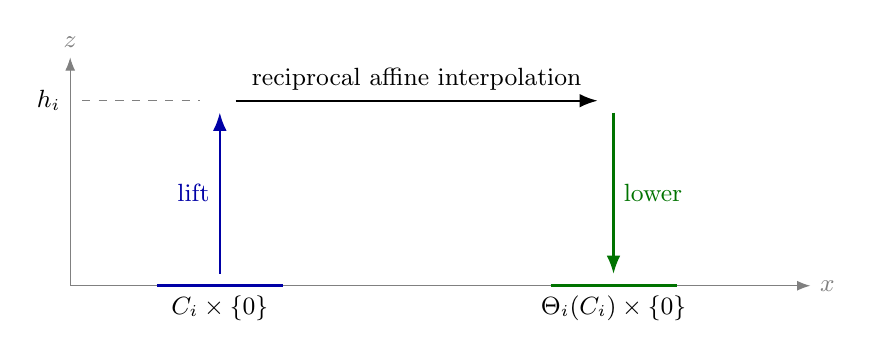
\begin{tikzpicture}[x=1cm,y=1cm,>=Latex,font=\small]
\draw[->,gray] (-.4,0)--(9,0) node[right] {$x$};
\draw[->,gray] (-.4,0)--(-.4,2.9) node[above] {$z$};
\draw[very thick,blue!65!black] (.7,0)--(2.3,0);
\draw[very thick,green!45!black] (5.7,0)--(7.3,0);
\node[below] at (1.5,0) {$C_i\times\{0\}$};
\node[below] at (6.5,0) {$\Theta_i(C_i)\times\{0\}$};
\draw[->,thick,blue!65!black] (1.5,.15)--(1.5,2.2)
 node[midway,left] {lift};
\draw[->,thick] (1.7,2.35)--(6.3,2.35)
 node[midway,above] {reciprocal affine interpolation};
\draw[->,thick,green!45!black] (6.5,2.2)--(6.5,.15)
 node[midway,right] {lower};
\draw[dashed,gray] (-.25,2.35)--(1.25,2.35);
\node[left] at (-.4,2.35) {$h_i$};
\end{tikzpicture}
\caption{The three scalar-potential phases for one instruction. This is a schematic projection onto the $x,z$ coordinates; the second planar coordinate is suppressed. Distinct branches use separate heights. Source rectangles are disjoint among themselves, as are image rectangles, while a source may overlap an image. During the middle phase the first coordinate stays between its endpoints.}
\label{fig:scalar-stages}
\end{figure}


For $m=1,2,3$ let $r_m(\tau)=\sigma(8\tau-(2m-1))$. The three derivative supports are disjoint and contained in $(0,1)$. Put
\[
 a_i(r)=1+(\lambda_i-1)r,\qquad b_i(r)=(\lambda_i-1)/a_i(r).
\]
For $(x_0,y_0)\in C_i$, the desired planar path is the reciprocal interpolation
\begin{equation}\label{bcs:scalar-path}
 (x,y)=(a_i(r)x_0+r\alpha_i,\ a_i(r)^{-1}y_0+r\beta_i),
 \qquad 0\le r\le1.
\end{equation}
It starts at $(x_0,y_0)$ and ends at $\Theta_i(x_0,y_0)$.
The scalar potential generating this path is
\[
 K_i(x,y,r)=b_i(r)xy+(1-rb_i(r))\alpha_i y
                         -(1+rb_i(r))\beta_i x.
\]
All denominators have a positive lower bound. Use the potentials
\begin{align*}
 P_1&=r_1' x\vartheta(z)\sum_i h_i g_i(x,y),\\
 P_2&=r_2'\Xi(x,y)\sum_i\eta_i(z)K_i(x,y,r_2),\\
 P_3&=-r_3' x\vartheta(z)\sum_i h_i\bar g_i(x,y),\qquad
 W=D_yP_1+D_zP_2+D_yP_3.
\end{align*}
The resulting field is divergence free, smooth, supported in one compact spatial set, and zero near the temporal endpoints.

For $(x_0,y_0)\in C_i$ at height zero, the first phase is exactly
$(x_0,y_0,h_i r_1)$. On this path $g_i=1$, all its derivatives vanish, and $\vartheta=1$, so the curl correction has no horizontal component. At height $h_i$ the second phase follows \eqref{bcs:scalar-path} with $r=r_2(\tau)$.
Indeed its derivatives with respect to $r$ are
$b_i x+(1-rb_i)\alpha_i$ and $-b_i y+(1+rb_i)\beta_i$, which are $\partial_yK_i$ and $-\partial_xK_i$. The choice of $A$ keeps the path in the plateau of $\Xi$; exactly one height cutoff is active. At its endpoint $\bar g_i=1$, so the third phase lowers it as $z=h_i(1-r_3)$. ODE uniqueness proves that these are the actual trajectories. One period therefore sends every point $(x,y,0)$ above $C_i$ to $(\Theta_i(x,y),0)$.

The first coordinate during \eqref{bcs:scalar-path} is
$(1-r)x_0+r\Theta_{i,1}(x_0,y_0)$. The other phases keep it fixed. Thus a branch with nonterminal endpoints cannot cross the negative detection half-space during its interpolation.

\subsection{Loading and an unbounded slow clock}
The initial code $(x_*,y_*)$ is rational because it has only finitely many nonblank digits. Put $r_*(t)=\sigma(2t-1/2)$ and, on $0\le t\le1$, use
\[
 P_*(t,x,y,z)=r_*'(t)\Xi(x,y)\vartheta(z)(x_*y-y_*x),\qquad U=D_zP_*.
\]
The trajectory of the origin is $(r_*x_*,r_*y_*,0)$. The chosen plateau contains this segment. Extend $W$ with period one in its time variable, writing the result as $V$. The loader occupies the first unit of time; after it, the onto processor clock $s=\log_2t$ starts at zero when $t=1$. For $t>1$ define
\[
 U(t,x)=\frac1{t\log2}V(\log_2t,x).
\]
The zero time collars glue these definitions smoothly at $t=1$. At $t=2^m$, the particle has the code after $m$ auxiliary steps, up to its first halt. This follows from the onto clock $\log_2t$ and the exact full-rectangle map. Each finite ordinary computation thus finishes in finite physical time.

For a nonhalting computation every code has $x\ge3$, and the loader travels from zero to such a code. Convexity of the first coordinate proves avoidance of $x<-1$ at every real time. A terminal code has $x\le-2$, including an initial halt immediately after loading. This proves the event equivalence.

Finally,
\[
 \partial_t[t^{-a}Y(\log_2t,x)]
 =t^{-a-1}[-aY+(\log2)^{-1}\partial_sY](\log_2t,x).
\]
The proof of Lemma~\ref{bcs:clock} therefore gives the stated $t^{-1-j}$ bounds on $t>1$; the finite loading interval adds bounded quantities. Define $f=U_t+(U\cdot\nabla)U-\nu\Delta U$. Fixed compact support gives the Sobolev comparison conditions and every asserted norm. Lemma~\ref{lem:b-comparison} proves uniqueness. All rules, cutoffs and clock formulas are finite effective data. Periodic evaluation uses a finite superset of possibly active translates, so it does not test equality at a seam or follow the machine's run. This proves Theorem~\ref{bcs:scalar-theorem}.

\section{Other clocks and spatial startup profiles}\label{bcs:clock-options}
The compact construction is now complete. We record optional root clocks and startup profiles. The logarithmic estimate in Lemma~\ref{bcs:clock} gains a factor $(1+t)^{-1}$ with each time derivative; the root-clock estimate below gives the common exponent $\beta$ at every fixed mixed order. The final profile proposition acts on a fixed spatial field $Z$, whose flow is autonomous, rather than on a time-dependent processor. Its force and trajectory identities also apply to the distinct startup profile $\sigma(t)$ used for the spatial suspension in Section~\ref{bcs:expanded-section}.

\begin{proposition}[The root clocks]\label{bcs:power-clock}
Under the hypotheses of Lemma~\ref{bcs:clock}, set $g(t)=(1+t)^q-1$, where $q=1/3$ or $q=1/4$, and put $\beta=1-q$. All mixed derivatives of the velocity and force in \eqref{bcs:clock-force} are bounded, and for every fixed $j,\alpha$,
\[
 \|\partial_t^jD_x^\alpha u(t)\|_\infty+
 \|\partial_t^jD_x^\alpha f(t)\|_\infty
 \le C_{j,\alpha}(1+t)^{-\beta}.
\]
In particular each is square-integrable in time in spatial supremum norm. The cube-root exponent is $2/3$ and the fourth-root exponent is $3/4$.
\end{proposition}
\begin{proof}
Every positive-order derivative $g^{(k)}$ is bounded and is $O_k((1+t)^{-\beta})$. Each differentiated term in $g'W(g)$ contains at least one such factor and a bounded derivative of $W$. One factor supplies the decay and the others are bounded. Applying this statement to $u_t-\nu\Delta u$, and applying the product rule to convection, proves the force estimate. Since $2\beta>1$, its square is integrable. Both clocks are increasing and unbounded, so Lemma~\ref{bcs:clock} applies to the event.
\end{proof}

The displayed bound applies to each mixed derivative separately; no claim of a common constant over all derivative orders is intended. An unslowed periodic field and any of these slowed fields define separate choices of force.

\begin{proposition}[A spatial field with a startup profile]\label{bcs:autonomous-profile}
Let $Z(x)$ be a smooth divergence-free field on a flat torus. Let $\sigma$ be the smooth step which is zero for $t\le0$, one for $t\ge1$, and satisfies $\sigma(t)+\sigma(1-t)=1$. Define
\[
 \alpha_0(t)=\sigma(2t-1),\qquad
 \alpha_1(t)=\frac{\sigma(2t-1)}{1+t},\qquad
 u(t,x)=\alpha(t)Z(x).
\]
For either choice $\alpha=\alpha_0,\alpha_1$, the residual force is
\begin{equation}\label{bcs:autonomous-force}
 f=\alpha'Z+\alpha^2(Z\cdot\nabla)Z-\nu\alpha\Delta Z.
\end{equation}
It has bounded mixed derivatives, gives zero initial velocity and pressure zero, and follows the spatial flow of $Z$ at the onto time $s(t)=\int_0^t\alpha$. For $\alpha_0$, $s(t)=t-3/4$ for $t\ge1$, and the force is stationary there. For $\alpha_1$,
\[
 s(t)=s(1)+\log\frac{1+t}{2}\quad(t\ge1),
\]
and the force tends uniformly to zero and belongs to space-time $L^2$. If $\int Z=0$, both forces have zero mean. In general their means equal $\alpha'\int Z$.
\end{proposition}
\begin{proof}
Substitution proves the force identity and the material correspondence. Symmetry of the step gives
$\int_0^1\sigma(2t-1)\,dt=\frac12\int_0^1\sigma(v)\,dv=1/4$.
The formulas for $s$ follow and show that its range is $[0,\infty)$. For the slow profile the coefficients $\alpha',\alpha^2,\alpha$ are respectively $O((1+t)^{-2})$, $O((1+t)^{-2})$, and $O((1+t)^{-1})$ after startup; all derivatives are bounded, and integration proves the force norm. Spatial integration of \eqref{bcs:autonomous-force} proves the mean statement.
\end{proof}

These elementary clock estimates do not give faster-than-every-power decay for an arbitrary repeated processor. For example, a nonnegative speed bounded by $C(1+t)^{-2}$ has finite accumulated time. The constructions with rapidly shrinking signals require their own memory mechanisms.

\section{Prefix histories and a plane that compensates area change}\label{bcs:prefix-section}
Reciprocal rectangle maps preserve planar area. Prefix replacements need not: writing a history symbol can change the total prefix length. We now allow arbitrary positive diagonal scalings in the plane, and compensate their area change in the transverse direction. The computational plane itself remains invariant. A logarithmic clock then gives a complete decaying-force construction from ordinary tape instructions.

\begin{theorem}\label{bcs:prefix-theorem}
For fixed computable $\nu>0$, every deterministic one-tape machine and finite input effectively determine a smooth mean-zero force on the unit torus, with zero initial velocity, such that
\[
 \|\partial_t^jD_x^\alpha f(t)\|_\infty\le C_{j,\alpha}(1+t)^{-1-j}
\]
for every $j,\alpha$. The unique global smooth velocity satisfies the same bounds. Its particle from $(1/4,1/2,1/2)$ enters $\{1/2<x_1<1\}$ exactly when the machine halts. One choice of force has pressure zero; projecting that force gives a divergence-free choice with the same velocity and a changed normalized pressure. For a fixed machine, the repeated motion before the clock change is independent of the input; only its initial loading motion changes.
\end{theorem}

\subsection{A record between ordinary tape symbols}
Let $Q$ be the finite state set, $q_{\mathrm{in}}$ its initial state, $Q_h\subseteq Q$ its terminal states, and $\Gamma$ the work alphabet with blank $\square$. Missing instructions are replaced by stationary transitions to an added terminal state, preserving the read letter. A transition into a terminal state is completed; an initially terminal configuration also counts as halting. Add a read-only origin bit to the work alphabet, one only at cell zero and preserved by every write. For empty input, the initial word is a marked blank. This allows recovery of the absolute head position after decoding.

The record symbols retain erased information in the sense of reversible history computation~\cite{Bennett1973}. For each nonterminal $q$, previous displacement $d\in\{-1,0,1\}$, and read letter $a$, create a record $g(q,d,a)$, and let $G$ be the set of these records. Two infinite stacks $L,R$ use the alphabet $\mathcal A=\Gamma\sqcup G$. Labels are $C(q,d)$ and $S_+(q),S_-(q)$. At a checkpoint $C(q,d)$, deleting the records from $L$ gives the tape left of the head in reverse order; deleting them from $R$ gives the tape from the head rightward. The top of $R$ is a work letter. The scan labels transfer leading records between the stacks until the next work letter appears.

A prefix rule $(\ell;\alpha,\beta)\to(\ell';\alpha',\beta')$ replaces the indicated prefixes of $L,R$ and retains their infinite tails. For $\delta(q,a)=(q',b,m)$ and $g=g(q,d,a)$, use
\begin{equation}\label{bcs:prefix-work-rules}
\begin{array}{lll}
 (C(q,d);\epsilon,a)\to(S_+(q');bg,\epsilon),& &m=1,\\
 (C(q,d);\epsilon,a)\to(S_-(q');\epsilon,bg),&&m=-1,\\
 (C(q,d);\epsilon,a)\to(C(q',0);g,b),&&m=0.
\end{array}
\end{equation}
Here $\epsilon$ is the empty word. For every $q$, every $g\in G$ and every $c\in\Gamma$, also use
\begin{equation}\label{bcs:prefix-scan-rules}
\begin{array}{ll}
 (S_+(q);\epsilon,g)\to(S_+(q);g,\epsilon),&
 (S_+(q);\epsilon,c)\to(C(q,1);\epsilon,c),\\
 (S_-(q);g,\epsilon)\to(S_-(q);\epsilon,g),&
 (S_-(q);c,\epsilon)\to(C(q,-1);\epsilon,c).
\end{array}
\end{equation}
The terminal labels are exactly the checkpoints $C(q,d)$ with $q\in Q_h$;
there are no rules out of them. The scan labels $S_\pm(q)$ remain
nonterminal even for $q\in Q_h$, so a pending move finishes before its
terminal checkpoint is reached. Initialize at $C(q_{\mathrm{in}},0)$ with
left stack $\square^\infty$ and right stack $\omega\square^\infty$, where
$\omega$ includes the origin bit.

\begin{lemma}\label{bcs:prefix-symbolic}
The full domain cylinders of these rules are pairwise disjoint, and their full image cylinders are pairwise disjoint. Initialized checkpoints recover the ordinary machine configurations. Each ordinary transition takes a positive finite number of prefix steps, and a terminal checkpoint occurs exactly on halting.
\end{lemma}
\begin{proof}
Rules with a common source label test incompatible top letters. For images entering $S_+(q)$, an ordinary transition begins the left stack with a work letter followed by its distinct source record, whereas a scan loop begins it with a record. These distinguish all incoming cylinders. The same argument uses the right stack for $S_-(q)$. Into $C(q,1)$ or $C(q,-1)$, the final scan writes a distinct first work letter on $R$; into $C(q,0)$, the source record at the start of $L$ distinguishes the rule. Labels separate the remaining cases. Thus these assertions hold for arbitrary tails, without an initialization assumption.

For a right move, \eqref{bcs:prefix-work-rules} removes the read letter from $R$ and puts the written letter and its record on $L$. The positive scan transfers leading records from $R$ until the next work letter is exposed. Deleting records gives exactly the rightward tape update. A left move first replaces the read letter by $bg$ on $R$; its scan transfers records from $L$ and then its first work letter to $R$, giving the leftward update. A stationary move only changes the scanned work letter after deletion. Each transition adds one record, so there are finitely many records at every reached checkpoint and every scan is finite. The origin bit survives deletion and gives absolute alignment. A scan associated to a transition into $Q_h$ finishes before the terminal checkpoint is declared. This proves the assertions, including initial halting.
\end{proof}

\subsection{A planar motion for arbitrary diagonal rectangle maps}
As in Moore's positional representation of symbolic shifts~\cite{Moore1991}, assign the ordered letters of $\mathcal A$ the digits $1,3,\ldots,2M-1$ in base $B=2M+1$, where $M=|\mathcal A|$. Set
\[
 \gamma(w)=\sum_{j\ge1}D(w_j)B^{-j},\quad
 c(\alpha)=\sum_{j=1}^{|\alpha|}D(\alpha_j)B^{-j},\quad
 I(\alpha)=[c(\alpha),c(\alpha)+B^{-|\alpha|}].
\]
The identity $\gamma(\alpha w)=c(\alpha)+B^{-|\alpha|}\gamma(w)$ and the gaps between digits prove unique decoding. Child intervals lie strictly inside the parent, so incompatible prefix cylinders have separated intervals even as closed sets.

Put $\Omega=(0,1)^2$ and $\Omega_-=(0,1/2)\times(0,1)$. If the labels number $N$, give label $\ell_i$ a square $K_i$ of half-side $1/[16(N+1)]$, centered at height $i/(N+1)$ and first coordinate $3/4$ for terminal labels, $1/4$ otherwise. Let $\Phi_i$ be the positive axis-preserving affine map of $[0,1]^2$ onto that square. The encoded state is
$\Phi_i(\gamma(L),\gamma(R))$. A rule with prefixes $\alpha,\beta$ and $\alpha',\beta'$ has rectangles
\[
 D_i=\Phi_\ell(I(\alpha)\times I(\beta)),\qquad
 E_i=\Phi_{\ell'}(I(\alpha')\times I(\beta')).
\]
Both families are separately disjoint by Lemma~\ref{bcs:prefix-symbolic}. Each source lies in $\Omega_-$, and each target lies entirely in one open half of $\Omega$. The positive diagonal affine map $D_i\to E_i$ implements the prefix rule exactly. Its determinant is allowed to differ from one.

The shrink--move--expand interpolation also appears in the proof of~\cite[Proposition~5.1]{CardonaMirandaPeraltaSalasPresas2021}; here we specify rational routes that preserve the required observation half-plane.

\begin{lemma}\label{bcs:prefix-planar}
Let $D_i,E_i$, $1\le i\le m$, be rational axis-aligned closed rectangles of positive side lengths. Suppose the $D_i$ are pairwise disjoint in $\Omega_-=(0,1/2)\times(0,1)$, the $E_i$ are pairwise disjoint in $\Omega=(0,1)^2$, and each $E_i$ lies entirely in one open half of $\Omega$. There is an effective smooth field $v_*(s,Y)$ supported in $(0,1)\times\Omega$ whose time-one map on each full $D_i$ is its positive diagonal affine identification with $E_i$. If $E_i\subset\Omega_-$, the whole trajectory from $D_i$ remains in $\Omega_-$. No incompressibility is asserted in this planar lemma.
\end{lemma}
\begin{proof}
For an empty list take zero. Otherwise choose positive rational enlargement margins separately for the source and target families, preserving their disjointness and their open-half containment. Let $p_i,q_i$ be their centers, and $r_i^D,r_i^E$ their half-side vectors. Write $y_0=\min_i\{p_{i,2},q_{i,2}\}$ and choose temporary centers
\[
 k_i=(1/8,\ i y_0/[2(m+1)]),\qquad 1\le i\le m.
\]
These are mutually distinct and lie below all source and target centers. Move $p_i$ to $k_i$ in increasing order, avoiding the centers $k_j$ with $j<i$ and $p_j$ with $j>i$. Then move $k_i$ to $q_i$ in increasing order, avoiding $q_j$ with $j<i$ and $k_j$ with $j>i$. Each first route stays in $\Omega_-$; a second route stays there if its target does, and otherwise stays in $\Omega$.

Here is a finite rational rule for such a route. In its allowed rectangle $(0,b)\times(0,1)$, choose a point $w$ at height $\min(p_2,q_2)/2$, off every line from either endpoint to a forbidden center. No horizontal forbidden line has this height. Each nonhorizontal line has one computable rational intersection with it. Choose $w_1$ positive and smaller than $b$ and every positive intersection coordinate, for example half their positive minimum with $b$. The two segments $p$--$w$--$q$ stay in the allowed rectangle and avoid the forbidden centers.

Choose a common rational $\varepsilon>0$ equal to $1/20$ times the minimum of the rectangle half-sides, segment-endpoint boundary distances, and, for each segment $a$--$b$ and forbidden center $o$, $|\det(b-a,o-a)|/2$; omit empty collections. Every included number is positive. Since segment lengths are less than two, the determinant quantity is a lower bound for the Euclidean distance to its line. The moving square of half-side $2\varepsilon$ therefore misses every stationary square of half-side $\varepsilon$: an intersection would put their centers within $3\sqrt2\varepsilon$, contradicting this clearance. It also remains inside its allowed rectangle.

Shrink each $D_i$ about $p_i$ to a square of half-side $\varepsilon$. To implement this, let $\zeta$ be a smooth step constant near the endpoints of $[0,1]$, put
\[
 A_i(\tau)=(1-\zeta(\tau))I+
       \zeta(\tau)\operatorname{diag}((\varepsilon,\varepsilon)/r_i^D),
\]
and multiply $A_i'A_i^{-1}(Y-p_i)$ by a cutoff equal to one near $D_i$ and supported in its chosen enlargement. The cutoffs are disjoint, all diagonal entries are positive, and the exact path is $p_i+A_i(\tau)(Y-p_i)$. The matrices shrink coordinatewise, so these paths stay in $D_i$.

For each scheduled segment $a$--$b$, put $c(\tau)=a+\zeta(\tau)(b-a)$ and use the translation field $c'(\tau)$ times a cutoff which is one on a neighborhood of the moving square and supported in the concentric square of half-side $2\varepsilon$. This translates that square exactly and vanishes on all held squares. After every small square has reached its target center, reverse the shrinking operation at each $q_i$ with matrices $(1-\zeta)I+\zeta\operatorname{diag}(r_i^E/(\varepsilon,\varepsilon))$. Its paths remain in $E_i$.

Each field vanishes near its phase endpoints. Rescale the finite list of $J$ phases $V_0,\ldots,V_{J-1}$ by $v_*(s)=J\sum_jV_j(Js-j)$ to fit them in one time unit. The resulting map sends $p_i+\xi$ to $q_i+\operatorname{diag}(r_i^E/r_i^D)\xi$, as required. Every stage obeys the indicated half-plane restriction. All cutoffs, paths, inverse diagonal lower bounds and derivative estimates are finite effective data.
\end{proof}

\subsection{Compensating the planar divergence}
The rational initial code is denoted by $Z_{\mathrm{in}}$. Its rationality follows from the finite input and the blank tail $D(\square)/(B-1)$. Let $p_*=(1/4,1/2)$ and load it along
$c(s)=p_*+\zeta(s)(Z_{\mathrm{in}}-p_*)$.
A translating bump supported in a sufficiently thin tube around this segment gives a field $v_{\mathrm{in}}$ with precisely that trajectory. For instance, take the half-side of the moving square to be one quarter of the smaller endpoint distance from $\partial\Omega$, and take the same enlargement margin. Convexity keeps the support in $\Omega$. A nonterminal loader stays in $\Omega_-$; a terminal loader reaches the right half.

Extend $v_*,v_{\mathrm{in}}$ by zero in time and periodically in space, and define
\[
 v(s,Y)=v_{\mathrm{in}}(s,Y)+\sum_{n\ge1}v_*(s-n,Y).
\]
All mixed derivatives are bounded because only one repeated phase template and one loader occur. At logical time $1+n$, the trajectory from $p_*$ is the code after $n$ prefix steps, up to a terminal visit. The rectangle lemma proves absence of a right-half visit during every nonterminal transition as well as at its endpoints. Together with the finite-scan invariant, this gives the all-time halting equivalence.

Choose a periodic smooth function $\eta(z)$ supported near $1/2$ which equals $z-1/2$ on a neighborhood of $1/2$. Define
\begin{equation}\label{bcs:prefix-lift}
 W(s,Y,z)=\bigl(\eta'(z)v(s,Y),-\eta(z)\operatorname{div}_Yv(s,Y)\bigr).
\end{equation}
The horizontal divergence and vertical derivative cancel. The spatial mean is zero: $\int\eta'=0$, and the integral of a periodic planar divergence is zero. At $z=1/2$, the vertical component vanishes and the horizontal component is exactly $v$. Thus this plane carries the entire prescribed computation despite the planar area changes. The lift has bounded mixed derivatives and vanishes at logical time zero.

Apply Lemma~\ref{bcs:clock} with $g(t)=\log(1+t)$. The particle from $(p_*,1/2)$ is $(Y(g(t)),1/2)$, so its prefix-step observations occur at $t=e^{1+n}-1$. Every finite logical time occurs at finite physical time, and the event equivalence is preserved. The lemma gives the exact derivative decay for the velocity and its residual, which has zero mean and pressure zero. Lemma~\ref{lem:b-comparison} gives uniqueness on the torus.

For clarity, the optional solenoidal force changes pressure. Given the residual $f$, let $\phi$ be the zero-mean solution of $\Delta\phi=\operatorname{div}f$ and replace $(f,p)$ by $(f-\nabla\phi,-\phi)$. This leaves $-\nabla p+f$ and therefore the velocity unchanged. In Fourier variables,
\[
 \phi(t,x)=-\sum_{k\ne0}\frac{i\,k\cdot\widehat f_k(t)}{2\pi|k|^2}e^{2\pi i k\cdot x}.
\]
Integration by parts in a coordinate of maximal $|k_l|$ gives, for every $m$,
$|\partial_t^j\widehat f_k(t)|\le C_{j,m}(1+t)^{-1-j}|k|_\infty^{-m}$.
There are $24r^2+2$ lattice points with $|k|_\infty=r$. Choosing $m$ large proves uniform convergence after any fixed derivatives, retains the decay, and gives effective tails. Finite Fourier coefficients are effectively integrated using derivative bounds. Termwise differentiation gives the Poisson equation, with zero mode zero; uniqueness of Fourier coefficients on continuous periodic functions identifies it pointwise. Thus the projected force is effective, mean zero and divergence free. This is the classical Helmholtz--Leray projection, with its pressure correction explicit.

Finally all infinite sums used to prescribe the force are evaluated from finite supersets of possibly active translates, obtained from a coarse enclosure of the time and position. The elementary flat-step derivatives have effective bounds near their seams. Neither construction nor evaluation uses a configuration reached after initialization. This completes Theorem~\ref{bcs:prefix-theorem}.

\paragraph{Other onto clocks.}
The field $W$ in \eqref{bcs:prefix-lift}, including its loader, also satisfies Proposition~\ref{bcs:power-clock}. Using $(1+t)^{1/3}-1$ or $(1+t)^{1/4}-1$ therefore gives separate force choices with the same fixed label and detector. Every mixed derivative is respectively $O((1+t)^{-2/3})$ or $O((1+t)^{-3/4})$. After the loader, the code after $n$ prefix steps is sampled at $(2+n)^3-1$ or $(2+n)^4-1$. These assertions use the same full-domain instruction motion and the same all-time path bound.

\section{A planar processor that leaves room for a spatial clock}\label{bcs:expanded-section}
The compact scalar-potential lift and the prefix lift spend the third coordinate on separating branches or compensating area change. For a stationary spatial suspension we instead need the entire instruction motion in a plane. We construct it by moving disjoint rectangles to well-separated temporary positions, changing their shapes there, and routing them to the targets. Input-dependent placement makes the initial particle fixed, so no one-time loader interrupts periodicity.

Fix
\[
 c_L=(1/4,1/4),\quad c_R=(3/4,1/4),\quad
 X_*=(1/4,1/4,1/4),\quad
 \mathcal S=\{X\in\mathbb T^3:2/3<X_1<5/6\}.
\]
We use the circle interpretation of the first-coordinate interval.

\subsection{A partial table with a recognizable inverse}
This construction retains an ordinary partial instruction table: the machine halts when its state and scanned letter have no instruction. The optional one-sided-tape convention of Section~\ref{bcs:scalar-section} is retained by including its immutable end-marker in the work alphabet and keeping the prescribed boundary actions; the recorder preserves that track. Let $Q$ be the finite state set, $A$ the work alphabet, $q_0$ the initial state, and $E\subset Q\times A$ the set of defined instructions, and write $e=(q,a)\mapsto(q'_e,b_e,d_e)$. Let
\[
 H_0=\{\mathtt u,\mathtt P\}\sqcup\{\mathtt r_e:e\in E\},
 \quad H_1=H_0\setminus\{\mathtt P\},\quad
 \Gamma=A\times H_0\times\{0,1\}.
\]
The extra tracks record instructions and mark the place to which the recorder must return, following the history principle of Bennett~\cite{Bennett1973}. States are ${\sf Run}_q,{\sf Turn}_q,{\sf Back}_q,{\sf Stop}_q$ and ${\sf Mark}_e,{\sf Seek}_e$. Put
\[
 (\tau_{q,a},\beta_{q,a},\mu_{q,a})=
 \begin{cases}({\sf Mark}_{(q,a)},b_{(q,a)},d_{(q,a)}),&(q,a)\in E,\\
 ({\sf Stop}_q,a,0),&(q,a)\notin E.
 \end{cases}
\]
At a checkpoint ${\sf Run}_q$ after $k$ ordinary steps, the intended invariant has frontier $F=2+k$ at least two cells to the right of the head, records in cells $2,\ldots,F-1$, blank history elsewhere except at the frontier, and all bits zero. Here a defined work instruction moves the head first; the next row marks that new position, scans right to append the record and advance the frontier, then returns to erase the mark. This order restores the updated head position at the next checkpoint, as the proof below shows.

Use exactly the following seven rule families:
\begin{equation}\label{bcs:expanded-table}
\begin{array}{lll}
 ({\sf Run}_q,(a,h,0))\mapsto(\tau_{q,a},(\beta_{q,a},h,0),\mu_{q,a}),&h\in H_1,\\
 ({\sf Mark}_e,(a,h,0))\mapsto({\sf Seek}_e,(a,h,1),1),&h\in H_1,\\
 ({\sf Seek}_e,(a,h,0))\mapsto({\sf Seek}_e,(a,h,0),1),&h\in H_1,\\
 ({\sf Seek}_e,(a,\mathtt P,0))\mapsto({\sf Turn}_{q'_e},(a,\mathtt r_e,0),1),\\
 ({\sf Turn}_q,(a,\mathtt u,0))\mapsto({\sf Back}_q,(a,\mathtt P,0),-1),\\
 ({\sf Back}_q,(a,h,0))\mapsto({\sf Back}_q,(a,h,0),-1),&h\in H_1,\\
 ({\sf Back}_q,(a,h,1))\mapsto({\sf Run}_q,(a,h,0),0),&h\in H_1.
\end{array}
\end{equation}
There are no rules out of a stop state. Initially the work tape is the finite input with blanks elsewhere, the head is at zero, every bit is zero, and the history has $\mathtt P$ at cell $2$ and $\mathtt u$ everywhere else.

\begin{lemma}\label{bcs:expanded-compiler}
The initialized table reaches a stop state exactly when the ordinary partial-table machine halts. Otherwise it has defined transitions forever. On its full allowed domain, the destination state and full written symbol determine a unique incoming rule; the destination alone determines its displacement.
\end{lemma}
\begin{proof}
At a checkpoint ${\sf Run}_q$ after $k$ ordinary steps, the state, head $i$, and work tape agree with the machine. The frontier is at $F=2+k$, records occupy $2,\ldots,F-1$, history is empty elsewhere, all bits are zero, and $i\le F-2$. A defined instruction first updates the work and moves to $i'=i+d_e\le F-1$. The mark row marks $i'$, the right scan reaches $F$, writes its record and moves to $F+1$. The turn row creates the new frontier and the backward scan finds the sole marked cell. Erasure restores the checkpoint invariant with $F$ increased by one. Each scan is finite. An undefined instruction enters a stop state by the first row, including at the initial configuration.

Into ${\sf Mark}_e$, $e$ identifies the old state and work letter, and the written history letter distinguishes the variants. Into ${\sf Seek}_e$ the marked entry and unmarked loop both move right and have different written bits. Into ${\sf Turn}_q$ the record identifies $e$. Into ${\sf Back}_q$ both arrivals move left; entry writes the frontier whereas the loop does not. Into ${\sf Run}_q$ the erasure row is the only type, and the written work and history letters recover its read symbol. Into ${\sf Stop}_q$ the unchanged letter identifies the old pair and the displacement is zero. Undoing that displacement and replacing the uniquely recovered read symbol reconstructs the full predecessor tape.
\end{proof}

\subsection{Coding a fixed starting point}
Give the $m=|\Gamma|$ letters odd digits $D(s)=1,3,\ldots,2m-1$ in base $B=2m+1$. Let
\[
 C(s_1s_2\cdots)=\sum_{j\ge1}D(s_j)B^{-j},\qquad
 I_s=[D(s)/B,(D(s)+1)/B].
\]
A code lies strictly inside its first-letter interval, and successive stripping uniquely decodes it. The left and right tape lists have coordinates $\xi=C(s_{-1}s_{-2}\cdots)$ and $\eta=C(s_0s_1\cdots)$. For a rule $(\varsigma,s)\mapsto(\tau,s',d)$ write $\beta=(D(s')-D(s))/B$. Its normalized rectangles and maps are
\begin{equation}\label{bcs:expanded-branches}
\begin{array}{ccl}
 d&\text{source}&(\xi,\eta)\longmapsto\\
 0&[0,1]\times I_s&(\xi,\eta+\beta),\\
 1&[0,1]\times I_s&((D(s')+\xi)/B,B\eta-D(s)),\\
 -1&I_l\times I_s&(B\xi-D(l),(D(l)+\eta+\beta)/B),\quad l\in\Gamma.
\end{array}
\end{equation}
The image rectangles are $[0,1]\times I_{s'}$, $I_{s'}\times[0,1]$, and $[0,1]\times(D(l)/B+B^{-1}I_{s'})$, respectively. The digit identities prove that these are the correct tape maps, with determinant one and positive diagonal part $\operatorname{diag}(B^{-d},B^d)$.

Let $K$ be the number of states and $N$ the number of split branches. They are positive, even if $E$ is empty, because the run-to-stop rules exist. Set
\[
 r=[10^6(K+1)(N+1)(B+1)^2]^{-1}.
\]
Each state has a square $o_\varsigma+r[0,1]^2$, based near $c_R$ for stop states and near $c_L$ otherwise. If $(\xi_*,\eta_*)$ is the rational initial tape code, set
$o_{{\sf Run}_{q_0}}=c_L-r(\xi_*,\eta_*)$.
Enumerate the other states by $j=1,\ldots,K-1$ and set their origins to their cluster base plus $(0,3jr)$. These squares are separated by at least $r$ and lie within sup distance $(3K+1)r$ of their bases. The initial physical code is exactly $c_L$.

Write the resulting physical affine branches $T_i:R_i\to R_i'$ with centers $p_i,p_i'$ and linear parts $\operatorname{diag}(\lambda_i,\lambda_i^{-1})$. Distinct sources are separated by at least $r/B^2$. Images have the same separation: in a target state the displacement is fixed and written symbols distinguish incoming rules, by Lemma~\ref{bcs:expanded-compiler}. For a left move, the two-digit target interval distinguishes $(l,s')$; its gaps are at least $B^{-2}$. This is a full-rectangle separation statement. At checkpoints, the record block length also recovers $k$, hence the frontier's absolute index $2+k$ and the absolute head position.

\subsection{Routing full rectangles inside the plane}
Area-preserving realization of symbolic rectangle maps is central to the generalized-shift construction of Cardona, Miranda, Peralta-Salas and Presas~\cite[Proposition~5.1]{CardonaMirandaPeraltaSalasPresas2021}. We give the full local construction needed here. Its quantitative collars and complete intermediate paths supply the later suspension and diffusion tests.
\begin{lemma}\label{bcs:expanded-processor}
There is an effective smooth planar Hamiltonian field $V(s,Y)$, period one in $s$ and zero near each integer phase, with support in $(1/8,7/8)^2$ and spatial mean zero, whose period map equals $T_i$ on each full $R_i$. All mixed derivatives have effective uniform bounds. A rectangle with a non-stop destination stays in $1/8<Y_1<3/8$ throughout its transition. The trajectory from $c_L$ enters $2/3<Y_1<5/6$ exactly when the machine halts, and a halting visit occurs at an integer phase.
\end{lemma}
\begin{proof}
Put $A_0=100B^2$ and expand source centers about $c_L$ to $P_i=c_L+A_0(p_i-c_L)$. Expand each target center about its own cluster base $c$ to $P_i'=c+A_0(p_i'-c)$. Within each family expanded centers are separated by at least $100r$, and they remain within $1/1000$ of their cluster bases. Choose temporary centers
$q_i=(1/4,3/4)+(0,100ir)$.
They too have separation $100r$, remain within $1/1000$ of $(1/4,3/4)$, and are far from either cluster.

Move the rectangles as
\[
 K_i(s)=c_i(s)+\operatorname{diag}(\theta_i(s),\theta_i(s)^{-1})(R_i-p_i).
\]
There are five operations: expand all source centers from $p_i$ to $P_i$ without changing shapes; move them one at a time to $q_i$; interpolate $\theta_i$ positively from $1$ to $\lambda_i$ there; move them one at a time to $P_i'$; and compress target centers about their cluster bases to $p_i'$. During the shape change each side length is monotone between its endpoint values and hence at most $r$.

Figure~\ref{fig:planar-routing} separates the roles of these five operations and shows the clearance used in the single-center moves below.
\begin{figure}[ht]
\centering
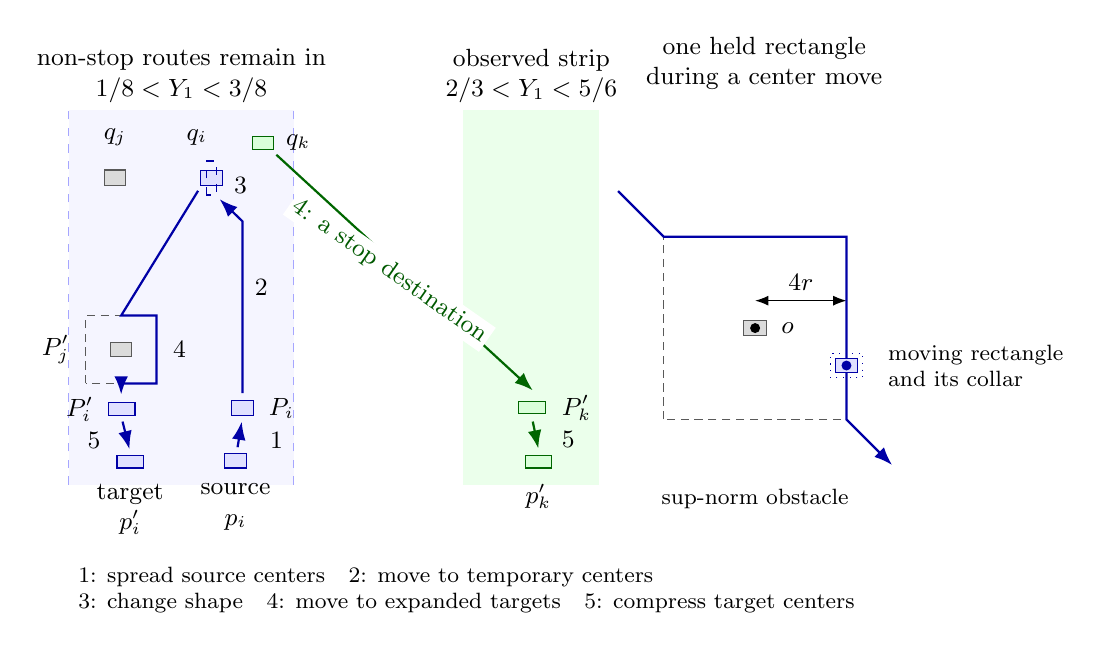
\begin{tikzpicture}[x=.88cm,y=.88cm,>=Latex,font=\small,
  move/.style={thick,blue!65!black,->},
  terminal/.style={thick,green!40!black,->},
  body/.style={draw=blue!65!black,fill=blue!12},
  held/.style={draw=black!65,fill=black!14}]
\fill[blue!4] (0,0) rectangle (3.25,5.4);
\draw[dashed,blue!35] (0,0)--(0,5.4) (3.25,0)--(3.25,5.4);
\node[align=center] at (1.63,5.9) {non-stop routes remain in\\$1/8<Y_1<3/8$};
\fill[green!8] (5.7,0) rectangle (7.65,5.4);
\node[align=center] at (6.68,5.9) {observed strip\\$2/3<Y_1<5/6$};
\draw[body] (2.25,.24) rectangle (2.57,.45);
\node[below,align=center] at (2.41,.15) {source\\$p_i$};
\draw[body] (2.35,1.0) rectangle (2.67,1.21);
\node[right] at (2.75,1.10) {$P_i$};
\draw[move] (2.44,.54)--(2.5,.91);
\node[right] at (2.77,.63) {1};
\draw[body] (.7,.24) rectangle (1.08,.42);
\node[below,align=center] at (.89,.15) {target\\$p_i'$};
\draw[body] (.58,1.0) rectangle (.96,1.18);
\node[left] at (.5,1.09) {$P_i'$};
\draw[move] (.78,.91)--(.88,.51);
\node[left] at (.6,.63) {5};
\draw[body] (1.90,4.32) rectangle (2.22,4.53);
\draw[blue!65!black,dashed] (1.99,4.18) rectangle (2.13,4.67);
\node[above] at (1.85,4.76) {$q_i$};
\node[right] at (2.25,4.32) {3};
\draw[held] (.52,4.32) rectangle (.82,4.54);
\node[above] at (.67,4.75) {$q_j$};
\draw[move] (2.51,1.32)--(2.51,3.8)--(2.18,4.12);
\node[right] at (2.55,2.85) {2};
\draw[held] (.61,1.85) rectangle (.91,2.05);
\draw[densely dashed,black!65] (.25,1.46) rectangle (1.27,2.44);
\node[left] at (.15,1.95) {$P_j'$};
\draw[move] (1.87,4.24)--(.76,2.44)--(1.27,2.44)--(1.27,1.46)--(.76,1.46)--(.76,1.30);
\node[right] at (1.37,1.95) {4};
\draw[draw=green!40!black,fill=green!15] (2.66,4.84) rectangle (2.96,5.02);
\node[right] at (3.0,4.93) {$q_k$};
\draw[terminal] (3.0,4.76)--(6.70,1.36);
\node[rotate=-35,fill=white,inner sep=1.3pt,text=green!35!black]
  at (4.63,3.08) {4: a stop destination};
\draw[draw=green!40!black,fill=green!15] (6.50,1.02) rectangle (6.88,1.20);
\node[right] at (6.98,1.11) {$P_k'$};
\draw[terminal] (6.70,.91)--(6.78,.52);
\node[right] at (6.98,.65) {5};
\draw[draw=green!40!black,fill=green!15] (6.59,.24) rectangle (6.97,.42);
\node[below] at (6.78,.15) {$p_k'$};
\node[align=left,anchor=north west,font=\footnotesize] at (0,-1.05)
  {1: spread source centers\quad 2: move to temporary centers\\
   3: change shape\quad 4: move to expanded targets\quad 5: compress target centers};
\begin{scope}[shift={(9.25,1.6)},x=.58cm,y=.58cm]
\node[align=center] at (1.2,6.8) {one held rectangle\\during a center move};
\draw[densely dashed,black!65] (-1,-1) rectangle (3,3);
\draw[held] (.75,.83) rectangle (1.25,1.17);
\fill (1,1) circle (1.8pt);
\node[right] at (1.36,1) {$o$};
\draw[<->] (1,1.6)--(3,1.6);
\node[above] at (2,1.6) {$4r$};
\draw[move] (-2,4)--(-1,3)--(3,3)--(3,-1)--(4,-2);
\draw[body] (2.76,.02) rectangle (3.24,.34);
\draw[blue!65!black,dotted] (2.65,-.09) rectangle (3.35,.45);
\fill[blue!65!black] (3,.18) circle (1.8pt);
\node[right,align=left,font=\footnotesize] at (3.7,.18) {moving rectangle\\and its collar};
\node[align=center,font=\footnotesize] at (1,-2.75)
  {sup-norm obstacle};
\end{scope}
\end{tikzpicture}
\caption{Planar routing, shown schematically with the small clusters and
rectangles magnified. A branch first moves to a temporary center, changes
shape there, and then moves to its target. A non-stop branch remains in the
left column; a branch with a stop destination may reach the observed strip.
The gray rectangle at $P_j'$ has already reached its expanded target and
is held during operation 4. The right inset distinguishes the center's
obstacle from the smaller held rectangle and the moving rectangle's collar.
Source and target clusters
may overlap, and routes used at different times may cross. The proof supplies
the quantitative separation and the schedule of moves; no distances are to scale.}
\label{fig:planar-routing}
\end{figure}


For a single-center move place a closed sup-norm square of radius $4r$ about each stationary center. These obstacles are disjoint: held centers belong to a temporary family and one expanded family, whose members have the stated separation. The endpoints avoid them. Start with the straight segment between the endpoints. Replace every portion inside an obstacle by the clockwise route along its boundary. The original crossing portions are disjoint by convexity; a detour meets no other obstacle because the squares are disjoint. Tangencies require no detour. This gives a finite rational polygonal path at sup distance at least $4r$ from each held center.

The paths lie well within the unit chart. For a move from source to temporary center they stay near the column $Y_1=1/4$. A move from temporary center to a non-stop target has endpoints within $1/1000$ of this column; its straight segment cannot meet a right-cluster obstacle, and its detours remain within $1/1000+4r$ of the column. Thus its entire rectangle stays in $(1/8,3/8)$ in the first coordinate. Moves to stop targets may cross the observed strip, as they should.

Divide $[0,1]$ into equal slots for all polygonal segments and each simultaneous expansion, shape change and compression. On each slot use the same smooth step $\zeta$ in its local time $\tau\in[0,1]$ for all interpolated quantities: a center moving from $a$ to $b$ follows $a+\zeta(\tau)(b-a)$, and each $\theta_i$ is interpolated with this step. In each simultaneous expansion or compression, center differences within a cluster are therefore multiplied by one common factor in $[1,A_0]$. These paths glue smoothly, and $\theta_i\ge B^{-1}$. Put $\varepsilon=r/(10B^2)$. The $\varepsilon$-enlargements of $K_i(s)$ remain disjoint. During source expansion, and during target compression within either cluster, a separating center difference is multiplied by a factor at least one while the rectangle sizes stay fixed.

\begin{samepage}
For targets in different clusters, both centers stay within sup distance $1/1000$ of their respective bases throughout compression. Their enlarged rectangles therefore have first-coordinate gap at least
\[
 1/2-2/1000-r-2\varepsilon>0.49.
\]
\end{samepage}

During routing the clearance $4r$ exceeds the sum of half-sides and collars; at temporary positions the separation is $100r$. They lie in $(1/8,7/8)^2$.

Choose a smooth product cutoff $\chi_i(s,Y)$ equal to one on the $\varepsilon/2$ enlargement and zero outside the $\varepsilon$ enlargement. With $Z=Y-c_i$ and $a_i=\dot\theta_i/\theta_i$, define
\[
 \psi_i=\chi_i(\dot c_{i,1}Z_2-\dot c_{i,2}Z_1+a_iZ_1Z_2),
 \qquad V=\sum_i(\partial_2\psi_i,-\partial_1\psi_i).
\]
On $K_i(s)$ this is exactly the affine velocity
$\dot c_i+\operatorname{diag}(a_i,-a_i)(Y-c_i)$.
Consequently the trajectory of every $Y_0\in R_i$ is
$c_i(s)+\operatorname{diag}(\theta_i,\theta_i^{-1})(Y_0-p_i)$ and ends at $T_i(Y_0)$. Disjoint collars eliminate interference. The compactly supported stream functions make the field divergence free with zero mean. Their vanishing time collars give a smooth periodic extension.

At integer phases the point from $c_L$ follows the table by induction. A stop code is near $c_R$ and lies in the strip; on a nonhalting run every destination is non-stop and the full continuous trajectory remains in the left column. Finally the finite rational geometry, positive denominator bound and explicit smooth cutoffs provide effective bounds at every derivative order, without executing the encoded machine.
\end{proof}

The same construction supplies the estimates needed for diffusion. Choose an effective integer $L\ge1$ bounding the first and second spatial derivative operator norms of $V$, and put $R=4^L$. If $\Psi_s$ is its flow from phase zero, then for $0\le s\le n$,
\begin{equation}\label{bcs:expanded-variation}
 \|D\Psi_s^{\pm1}\|_\infty\le e^{Ln}\le R^n,
 \qquad \|D^2\Psi_s^{\pm1}\|_\infty\le nLe^{3Ln}\le nLR^{3n}.
\end{equation}
Indeed the first variation equation has coefficient norm at most $L$. The second has the same linear coefficient, zero initial data, and forcing at most $L$ times the square of the first variation; variation of constants gives the bound. The reversed-time field has the same spatial derivative bounds, proving the inverse estimates as well.

\subsection{Periodic and eventually stationary forcing}
\begin{proposition}\label{bcs:expanded-material}
For each fixed computable $\nu>0$, the machine and input effectively determine a smooth period-one mean-zero force on $\mathbb T^3$, all of whose derivatives are bounded, such that the solution from zero velocity has its particle from $X_*$ enter $\mathcal S$ exactly when the machine halts. A separate choice of force is stationary for $t\ge1$, also with bounded derivatives and the same fixed event. Both constructions have pressure zero. The stationary choice has a generally nonzero mean force during startup.
\end{proposition}
\begin{proof}
For the periodic choice take $U(t,X)=(V(t,(X_1,X_2)),0)$ and its residual. The phase collar makes $U(0)=0$. Its mean is zero, all derivatives are bounded, and the fixed particle has constant third coordinate $1/4$. Lemma~\ref{bcs:expanded-processor} proves the event; Lemma~\ref{lem:b-comparison} gives uniqueness. The optional torus projection may make this periodic force solenoidal, with its accompanying pressure change.

Spatial suspension is the standard way to turn a periodic motion into an autonomous one; see Moore~\cite[Section~6]{Moore1991} and the geometric construction in \cite[Theorem~3.1]{CardonaMirandaPeraltaSalasPresas2021}. In the present flat coordinates the formula and its startup mean are explicit. For the stationary choice put
\[
 Z(X)=(V(X_3-1/4,(X_1,X_2)),1),\qquad U(t,X)=\sigma(t)Z(X).
\]
Periodicity in the phase makes $Z$ smooth on the torus, and its divergence is zero. Its residual is
$\sigma'Z+\sigma^2(Z\cdot\nabla)Z-\nu\sigma\Delta Z$,
which is stationary after time one. Set $s(t)=\int_0^t\sigma$. The particle's third coordinate is $1/4+s(t)$ modulo one, and its planar coordinates are $\Psi_{s(t)}(c_L)$. The clock is onto, so the same event equivalence follows. Here $\int Z=(0,0,1)$, hence
\[
 \int U=(0,0,\sigma(t)),\qquad \int f=(0,0,\sigma'(t)).
\]
The vertical startup acceleration therefore contributes the mean force shown above; after startup that mean is zero.
\end{proof}

\subsection{A velocity threshold for the same strip}\label{bcs:expanded-diffusion}
The injection, stirring and waiting theorem in \cite[Theorem~3.1]{velocity2026} applies to this planar field. Each block injects a fresh narrow scalar bump near $c_L$, carries it through $n$ processor periods in a short physical interval, and then lets heat diffuse during a long wait. The short stirring time keeps the new bump close in height to its transported profile; its small mass and the waits keep old injections below the detection threshold. The scalar becomes the third velocity component, so a visit of a transported bump to the strip yields a velocity-field observation. We now state the exact substitution and the bounds supplied by that theorem.

Take its initial point to be $c_L$, its observed planar set to be $E=\{2/3<Y_1<5/6\}$, and its constants to be $d=1/16$ and $C_H=10^8$. The field $V$ is Hamiltonian, smooth, period one, has zero phase collars and a fixed compact chart support. Lemma~\ref{bcs:expanded-processor} gives a terminal integer-phase visit, which is precisely the companion theorem's halting hypothesis; the constant $d$ controls the nonhalting separation below. In a nonhalting run the trajectory lies in $1/8<Y_1<3/8$, whose infimum circle distance from the observed arc is
\[
 \min\{2/3-3/8,\ 1+1/8-5/6\}=7/24>2d.
\]
Thus the whole nonhalting orbit has distance at least $7/24>2d$ from $E$. Equation~\eqref{bcs:expanded-variation} supplies the effective forward and inverse first and second derivative bounds. These verify every geometric hypothesis of the parameterized compact detector theorem.

For specificity, its unit-viscosity construction uses $R=4^L$, a smooth bump $g$ supported in $[-1,1]^2$, equal to one near zero and between zero and one, and a bound $C\ge1$ on its first two derivative operator norms. All derivative norms here are Euclidean operator norms, as in the companion theorem. Its parameters here are
\begin{align*}
 b_n&=10^{-6}(2R)^{-n},&g_n(Y)&=g((Y-c_L)/b_n),\\
 D_n&=2Cb_n^{-2}(1+nL)R^{3n},&\delta_n&=[100(1+D_n)]^{-1},\qquad t_n=2n.
\end{align*}
Here $D_n$ bounds the Laplacian of the bump after transport through at most $n$ periods; the choice of $\delta_n$ controls the accumulated diffusion error.
If $V_0$ is one period extended by zero, the prescribed horizontal field and scalar source are
\[
 a(t,Y)=\sum_{n\ge1}\frac n{\delta_n}\sum_{j=0}^{n-1}
 V_0\left(\frac{n(t-t_n-\delta_n)}{\delta_n}-j,Y\right),\qquad
 h(t,Y)=\sum_{n\ge1}\delta_n^{-1}\sigma'((t-t_n)/\delta_n)g_n(Y).
\]
Let $F=a_t+(a\cdot\nabla)a-\Delta a$. The force is the precomputed pair $(F,h)$; the unknown transported scalar is absent from it. The theorem supplies the scalar $w$ solving $w_t+a\cdot\nabla w=\Delta w+h$, $w(0)=0$, and the velocity $(a,w)$ with pressure zero. In this specialization, the total injected mass is bounded by $M_0$, with
\[
 M_0=\sum_{n\ge1}4b_n^2<10^{-11},\qquad
 2\delta_nD_n<1/50<1/16,\qquad 2-2\delta_n>1.
\]
The companion theorem uses these inequalities with the off-diagonal heat bound $C_H=10^8$ at separation $1/16$. It proves an all-time velocity threshold, including the waits between bursts, rather than only a sampled-time statement.

\begin{corollary}\label{bcs:expanded-eulerian}
For fixed computable $\nu>0$, the machine and input effectively determine a smooth prescribed force on $[0,\infty)\times\mathbb T^3$, whose unique global smooth solution from zero velocity and with pressure zero satisfies
\[
 \exists t\ge0\ \exists X\in\mathcal S:\ u_3(t,X)>1/2
 \quad\Longleftrightarrow\quad\text{the machine halts}.
\]
Uniqueness holds in the torus classical comparison class of Section~\ref{sec:analytic}: the velocity, its time derivative and spatial derivatives through order two are continuous on each finite closed cylinder, and the periodic pressure and its gradient are continuous, with mean-zero pressure normalization. No uniform large-time amplitude bound or mean-zero condition is asserted for this force.
\end{corollary}
\begin{proof}
The verified substitution in \cite[Theorem~3.1]{velocity2026} gives the unit-viscosity assertion. For general viscosity set
\[
 U_\nu(t,Y,z)=(\nu a(\nu t,Y),w(\nu t,Y)),\qquad
 f_\nu(t,Y,z)=(\nu^2F(\nu t,Y),\nu h(\nu t,Y)).
\]
Independence of $z$ makes each horizontal equation acquire factor $\nu^2$ and the scalar equation factor $\nu$. Thus the equations have viscosity $\nu$ and pressure zero, while the observed third component keeps threshold $1/2$. Finite-time smoothness, effectivity and uniqueness are exactly the conclusions of the invoked detector theorem and Lemma~\ref{lem:b-comparison}.
\end{proof}

\paragraph{The material event during the diffusion experiment.}
The same force also retains the fixed material event from $X_*$. At unit viscosity, block $n$ advances the horizontal flow through $n$ full processor periods and each gap freezes the horizontal position. Let $S(t)$ be the cumulative processor time: it is zero before the first stirring interval, increases from $n(n-1)/2$ to $n(n+1)/2$ in block $n$, and is constant between stirring intervals. More explicitly, in the stirring interval of block $n$ put
\[
 \tau=\frac{n(t-t_n-\delta_n)}{\delta_n}\in[0,n],\qquad
 S(t)=\frac{n(n-1)}2+\tau.
\]
The preceding cumulative phase is an integer. Periodicity gives $V(\tau,Y)=V(S(t),Y)$, so $a(t,Y)=S'(t)V(S(t),Y)$ inside each burst. During injections and waits, $a=0$ and $S$ is constant. The zero phase collars and continuity join these identities at the endpoints. Uniqueness therefore gives the horizontal trajectory $\Psi_{S(t)}(c_L)$, including partial bursts. The horizontal field is independent of the third coordinate, so the vertical motion driven by $w$ does not change this identity. The function $S$ is continuous, nondecreasing, finite at finite time, and unbounded. Lemma~\ref{bcs:expanded-processor} therefore proves entry into the original strip exactly on halting, including throughout the bursts and gaps. At viscosity $\nu$, use $S(\nu t)$. The scalar injections independently begin at $c_L$ and test successively longer prefixes; they do not reset the material trajectory.


\section{The decision consequence and exact observation}\label{sec:decision}
\begin{corollary}
There is no algorithm deciding the fixed material reachability event from every force description produced by Theorem~\ref{bcs:scalar-theorem}. The same conclusion holds separately for the force descriptions and fixed observations of Theorem~\ref{bcs:prefix-theorem}, Proposition~\ref{bcs:expanded-material}, and Corollary~\ref{bcs:expanded-eulerian}.
\end{corollary}
\begin{proof}
Compose a proposed decision algorithm with the effective construction from a machine and input. The proved equivalence between the event and halting would decide whether that arbitrary machine halts. Turing's symbol-printing undecidability gives the contradiction after the elementary modification described in the introduction~\cite[Section~8]{Turing1936}.
\end{proof}

The constructions use exact real positions and exact force prescriptions. Their conclusions concern the complete trajectory or velocity at every real time. A uniform tolerance for perturbing the program, the field or the observed coordinates is a separate requirement. Likewise, an onto slowdown preserves every finite computational step but does not furnish faster-than-every-power decay for an arbitrary periodic mechanism. These distinctions specify what the fixed detectors and slow clocks prove.

\bibliographystyle{plain}
\bibliography{references}
\end{document}
